\chapter{Propostas}
\label{cha:propostas}

Esse capítulo tem como base as oportunidades, fraquezas e ameaças do programa Ocean levantados no capítulo anterior, e tem como objetivo definir e criar uma proposta de desenvolvimento para um deles. Embora todos os pontos sejam levados até a gestão PRO/Samsung, foram realizado um critério de priorização de forma a selecionar os mais relevantes para serem desenvolvidos.

\section{Análise das oportunidades, fraquezas e ameaças}

De forma a facilitar a priorização dos pontos a serem trabalhados, as oportunidades, fraquezas e ameaças foram agrupadas em 4 categorias, explicadas a seguir: 

\begin{description}

\item[Pontos "passivos"] - Alguns pontos levantados não geram nenhuma ação a ser realizada por parte da gestão do laboratório, pois a gestão já permite o seu desenvolvimento, só faltando oportunidades ou resultados que aparecerão com o tempo. Entre esses pontos estão "Utilização do laboratório para a pós-graduação, na geração de pesquisas", "Maior utilização do laboratório em aulas do departamento", "Expansão dos projetos e parcerias (NEU) além dos cursos intensivos" e "Instituições de aceleração de empresas não-gratuitas podem tentar entrar na universidade". Os três primeiros pontos não apresentam nenhuma barreira para se desenvolverem naturalmente, e são fatores que a gestão acompanhará de perto. O último é considerado pela gestão improvável de acontecer pois com o aumento de instituições de aceleração oferecendo cursos bons gratuitos dentro da universidade, as instituições pagas têm menos incentivo para querer entrar na universidade.

\begin{figure}[H]
\caption{Pontos Passivos}
\centerline{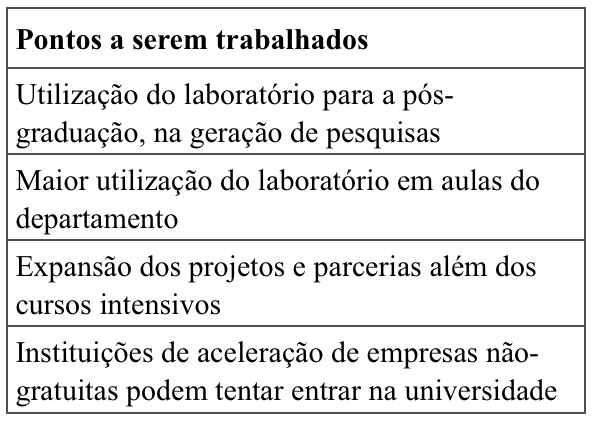
\includegraphics[scale=0.75]{img/pontosselecionadospassivos}}
\label{fig:pontosselecionadospassivos}
\caption* {Fonte: Elaborado pelo próprio autor}
\end{figure}

\item[Pontos levantados pelos cursistas] - Em relação aos pontos levantados sobre \textit{feedbacks} dos cursistas, será elaborado um relatório executivo com menor teor acadêmico porém mais detalhes diante das análises realizadas. Em relação aos cursos básicos, poderá será feita uma segmentação dos \textit{feedbacks} por ano de realização do questionário ou por tipo de curso dado pelo laboratório. Já para os cursos intensivos, poderão ser explorados os pontos levantados do ponto de vista de cada grupo, incluindo a identificação de 'frases de efeito' que poderiam ser utilizadas em um material de divulgação do curso. Não obstante, como esses pontos devem ser trabalhados quase que exclusivamente pela gestão da Samsung, serão levantadas questões a respeito de como desenvolver esses pontos, porém eles apresentam pouca prioridade para os fins deste trabalho.

\begin{figure}[H]
\caption{Pontos levantados pelos cursistas}
\centerline{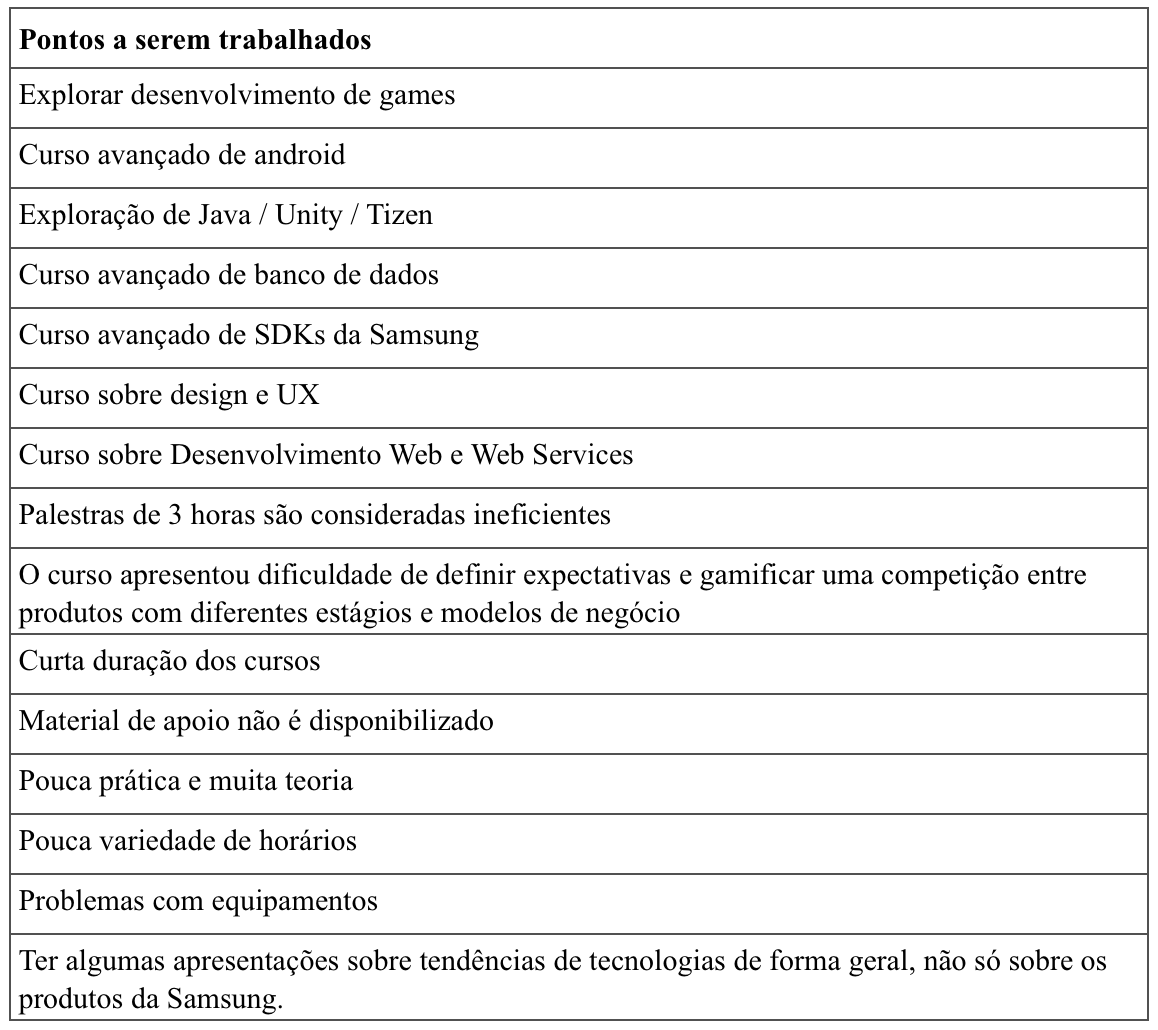
\includegraphics[scale=0.75]{img/pontosselecionadoscursistas}}
\label{fig:pontosselecionadoscursistas}
\caption* {Fonte: Elaborado pelo próprio autor}
\end{figure}

\item[Pontos considerados operacionais] - Os pontos operacionais são aqueles que podem ser corrigidos com alguma ação a ser tomada sem a necessidade de tomar algum decisão considerada estratégica pela gestão. Dentro desses pontos estão "Falta de conhecimento sobre os programas do laboratório", "Falta de instruções sobre o processo de utilização" e "Falta de agenda pública com os compromissos do Ocean". São pontos relevantes, e a gestão deverá fazer algo a respeito deles para maximizar o uso do laboratório pelos alunos.

\begin{figure}[H]
\caption{Pontos operacionais}
\centerline{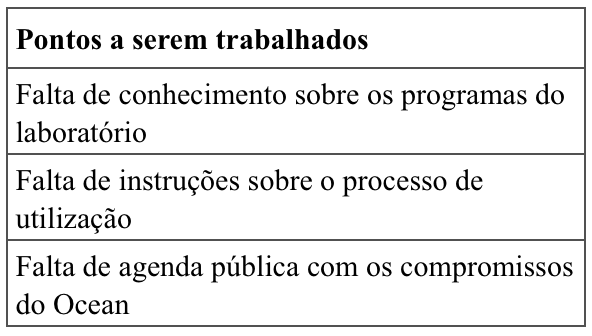
\includegraphics[scale=0.75]{img/pontosselecionadosoperacionais}}
\label{fig:pontosselecionadosoperacionais}
\caption* {Fonte: Elaborado pelo próprio autor}
\end{figure}

\item[Pontos estratégicos] - Os pontos considerados mais estratégicos são aqueles que podem ser desenvolvidos e transformados em projetos de curto, médio ou longo prazo, e têm potencial de trazer um impacto muito positivo para o Ocean.

\begin{figure}[H]
\caption{Pontos estratégicos}
\centerline{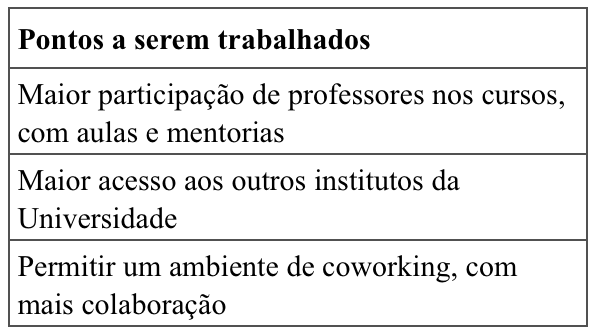
\includegraphics[scale=0.75]{img/pontosselecionadosestrategicos}}
\label{fig:pontosselecionadosestrategicos}
\caption* {Fonte: Elaborado pelo próprio autor}
\end{figure}

\end{description}

Definidas as categorias, foram definidos níveis de priorização para cada uma, juntamente com a gestão do laboratório Ocean. Foram atribuídas as notas 1, 3, 5 e 7 para as categorias, sendo a nota 1 os pontos prioritários e o 7 o de menor prioridade.


\begin{figure}[H]
\caption{Priorização de pontos}
\centerline{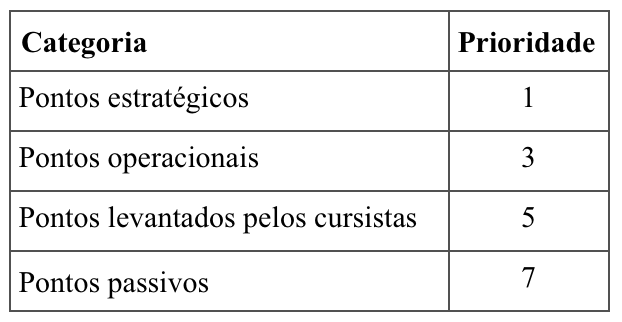
\includegraphics[scale=0.75]{img/priorizacao}}
\label{fig:priorizacao}
\caption* {Fonte: Elaborado pelo próprio autor}
\end{figure}

\section{Desenvolvimento dos pontos prioritários}

Cada um dos pontos prioritários será desenvolvido através de um estudo de possíveis soluções e levantamento das principais dificuldades de implementação.

\subsection{Maior participação de professores nos cursos}

Segundo a gestão do Ocean, a participação de professores nas frentes de ensino dos cursos enriqueceria o conteúdo transmitido, pois fornece uma base teórica que em si justifica grande parte dos métodos utilizados atualmente de forma empírica. Não obstante, a grande variedade de cursos superiores entre os participantes dos programas intensivos têm como consequência pessoas que têm bastante conhecimento sobre certas metodologias e outras que tiveram pouco ou nenhum  contato com as mesmas, o que dá espaço para um professor especialista reafirmar um assunto para os especialistas e abrir novos horizontes para os menos experientes. 

A Universidade de São Paulo possui grandes educadores em todos os seus institutos, e em especial o IME, FEA e as faculdades da Poli possuem professores especialistas em criação e desenvolvimento de produtos, inovação e empreendedorismo, que trariam muito conhecimento para os cursistas e para o programa. Entretanto, como a participação de professores nos cursos ainda não ocorre com muita frequência, seria prudente começar a intensificação desse tipo de parceria pelo PRO, pois se mantém a facilidade de comunicação entre o laboratório e o departamento, sem uma necessidade de modificar ou estruturar os processos atuais de funcionamento e comunicação do Ocean.

Considerando a grade de ensino da Engenharia de Produção da Poli, observa-se que muitas disciplinas possuem uma sinergia muito grande com a proposta de pré-aceleração de empresas do laboratório: 

\begin{description}
\item[Projeto Integrado de Sistemas de Produção] - tem como objetivo "Estabelecer uma ponte entre a formação acadêmica e o mundo profissional, com foco no planejamento, elaboração e implantação de projetos e novos empreendimentos", e introduz muitos conceitos como planos de modelo de negócio - guiado principalmente pelo \textit{Canvas} - e fontes de captação de recursos, como "Venture Capitals" e "Private Equities"

\item[Projeto do Produto e Processo] - segmenta o processo de desenvolvimento de um produto em diversas etapas de validação, "Concepção do Produto", "Avaliação do preço do produto", "Desenvolvimento do Produto", "Desenvolvimento dos Desenhos de Engenharia", "Resolução do Processo", "Sistema de informação e Layout", "Viabilidade Comercial e Engenharia de Valor"

\item[Projeto, Processo e Gestão da Inovação] - discute como empresas devem se organizar para facilitar e fomentar a gestão da inovação para criar oportunidades de negócios, através da criação e acompanhamento de projetos-chave e da definição de proessos e KPIs para os seus principais objetivos.

\end{description}

Muitas outras disciplinas ainda apresentam conceitos interessantes que poderiam ser utilizados em um escopo menor do que o apresentado na disciplina, como a "Gestão de Projetos" e "Princípios de Marketing para Engenharia de Produção", ilustrando a possível sinergia entre os professores do departamento e o laboratório Ocean através do conteúdo ensinado em aula para os alunos do PRO.

Embora toda essa sinergia evidencie o quanto os professores podem enriquecer os cursos do Ocean, ela não é suficiente para garantir uma maior participação de professores nos cursos, pois embora o laboratório seja de cogestão do PRO os cursos são geridos pela Samsung, o que traz algumas complicações para essa parceria. Os cursos normalmente possuem horário incompatível com a grade horária dos professores, o escopo do trabalho dos professores já está bem definido, e por ser um projeto inicial, não há muito investimento dos professores planejado com o laboratório. No entanto, sabe-se que por a Samsung ser uma empresa externa à universidade, a parceria com os docentes poderia ser facilitada através do financiamento de palestras, aulas e mentorias, o que é inexistente no momento.

Em conversa com Selber, gestor da unidade Ocean, foi discutida a possibilidade de financiamento dos professores, e a barreira existente para isso acontecer está na organização da Gestão Financeira da \textit{Samsung} diante dos recursos separados para a Lei da Informática.


\subsection{Maior acesso aos outros institutos da universidade}
\subsection{Permitir um ambiente de \textit{coworking}, com mais colaboração}

Os dois primeiros pontos em questão estão sendo avaliados pelo departamento, pois envolvem uma remuneração extra para os professores participarem nesses cursos e uma maior divulgação do laboratório por parte de todos os \textit{stakeholders}, principalmente o NEU e o PRO. Portanto juntamente à gestão do PRO e da Samsung, foi definido que seria desenvolvido o terceiro ponto mencionado, \textbf{"Permitir um ambiente de \textit{coworking}, com mais colaboração"}, pois além de ser uma questão estratégica para o laboratório, ele pode evitar o problema de o laboratório se tornar uma biblioteca ou uma pró-aluno.
